\documentclass[singlespacing, latexmargins]{ludis}

% % custom packages by Peteris Ratnieks
\usepackage{booktabs}
\usepackage{listings}
\lstset{numbers=left,
    stepnumber=1,
    firstnumber=1,
    numberfirstline=true
}
% \lstinputlisting[language=Python, firstline=2, lastline=22]{code.py}

% XeLaTeX atbalsts tiek pieslēgts ar šādām pakotnēm:
\usepackage{fontspec}
\usepackage{xunicode}
\usepackage{xltxtra} %

% Valodu atbalsts
\usepackage{polyglossia}
\setdefaultlanguage{latvian}
\setotherlanguages{english,russian}

% Fonti -- var rakstīt sistēmas fontu nosaukumus
% \setmainfont[Mapping=tex-text]{Times New Roman}
% \setsansfont[Mapping=tex-text]{Arial}
% \newfontfamily\russianfont{Times New Roman}

\usepackage{multirow}

\usepackage{hyperref}


\def\r{\mathbb{R}}
\def\n{\mathbb{N}}

\def\m{\mathcal{M}}
\def\k{\mathcal{K}}
\def\a{\mathcal{A}}
\def\s{\mathcal{S}}

\def\sumin{\sum_{i=1}^n}
\def\sumon{\sum_{i=0}^n}
\def\suminf{\sum_{i=1}^\infty}
\def\ppt{\textsf{PPT}}
\def\t{\textsf{T}}
\def\f{\textsf{F}}
\def\oi{\{0,1\}}

\newcommand{\bra}[2]{\langle #1,#2 \rangle}


\fakultate{Fizikas, Matemātikas un Optometrijas}
\nodala{Fizikas}
\nosaukums{Title}
\darbaveids{Bakalaura}
\DARBAVEIDS{BAKALAURA}
\autors{Viktorija Leimane}
\studapl{vl16047}
\vaditajs{Vadītājs}
\recenzents{Recenzents}
\vieta{Rīga}
\gads{2019}


\begin{document}

\maketitle

\begin{abstract-lv}
Darba mērķis ir noteikt efektīvāko saules paneļu izvietojuma veidu Latvijai tipiskos meteoroloģiskajos apstākļos. 
Balstoties uz divu veidu saules paneļiem, kas novietoti piecās dažādās telpiskajās orientācijās Latvijas Universitātes Botāniskā dārza teritorijā, tiks noteikta solāro paneļu efektivitātes atkarība no mainīgiem parametriem:
1) meteoroloģiskie apstākļi
2) telpiskā orientācija
3) gada mēnesis
4) solāro paneļu tips. \\
Iegūtie monitoringa rezultāti tiks analizēti kontekstā ar šo paneļu efektivitātes fizikālo novērtējumu.\\

\keywords{Saules enerģijas paneļi, atjaunojamo energoresursu enerģija, vides monitorings}
\end{abstract-lv}

\begin{abstract-en}
The aim of this thesis is to determine the most efficient way of solar panel arrangement for typical weather conditions in Latvia.
Based on two types of solar panels placed in five different spatial orientations in the University of Latvia Botanical Garden area, the dependency of the efficiency of solar panels on following variable parameters will be established:
% or determined
1) meteorological conditions
2) spatial orientation
3) month of year
4) type of solar panels.\\
The results of monitoring will be analyzed in the context of a physics based assessment of the effectiveness of these panels.\\

\keywords{Solar panels, renewable energy, environmental monitoring}
\end{abstract-en}

\tableofcontents

\specnodala{Apzīmejumi}
\begin{description}
    % \item[\ppt] Varbūtisks algoritms
    % \item[Ķēde] Decentralīzēta publiski pieejama datu bāze, kas darbojas pēc saviem noteikumiem.
\end{description}


\specnodala{Ievads}
Apvienoto Nāciju Organizācijas Klimata konferencē Parīzē 2015. gada decembrī daudzas pasaules valstis vienojās ierobežot globālo sasilšanu zem 2 ºC salīdzinājumā ar pirmsindustriālo laikmetu.
%, tāpēc ES ir apņēmusies līdz 2030. gadam samazināt siltumnīcefekta gāzu emisijas vismaz par 40\% salīdzinājumā ar 1990. gada līmeni.
Tāpēc Eiropas Savienībā noteikts dalībvalstīm saistošs mērķrādītājs  –  vismaz 32\%  atjaunojamās enerģijas īpatsvars līdz 2030. gadam \cite{ES}.

Ne mazāk būtiska ir atjaunojamo energoresursu loma energoapgādes neatkarības un drošības veicināšanā, tehnoloģiju attīstībā un inovācijās, vienlaikus sniedzot labumu videi un sabiedrībai, kā arī nodrošinot svarīgus priekšnosacījums nodarbinātībai, reģionālajai attīstībai un elektrības nodrošināšanai grūti pieejamās vietās \cite{ES}.

Dažādu pieejamo atjaunojamo resursu - Saule, vējš, zeme, ūdens - starpā Saules enerģija ir viens no kandidātiem klimata pārmaiņu un to seku mazināšanai un efektīvas energoapgādes nodrošināšanai. Pēdējā desmitgadē veiktās investīcijas Saules enerģijas izmantošanā manifestējās inovācijās saules paneļu ražošanā, un gala rezultātā tie ir kļuvuši efektīvāki un finansiāli pieejamāki patērētājiem, piemēram, rakstā \cite{researchOpp} norādīts, ka silīcija saules paneļu cena sastāda mazāk nekā 30\% no kopējām saules paneļu sistēmas uzstādīšanas izmaksām un to saražotā enerģija atmaksājas vidēji trīs gadu periodā.

Tomēr bez klimata to efektivitāti ietekmē arī daudzi citi faktori, to skaitā telpiskā orientācija.

Šī pētījuma \textbf{mērķis} ir analizēt un praktiski pārbaudīt divu tipu (JA un LG) saules paneļu efektivitāti atšķirīgos telpiskās orientācijās risinājumos -- pētītas trīs dažādu virzienu (dienvidi, rietumi, austrumi) un trīs leņķu (13, 40, 90) paneļu grupas -- un tiek salīdzināta to piemērotība Latvijas klimatiskajiem apstākļiem.

\textbf{Darba uzdevumi}
\begin{itemize}
\item Ievākt, atlasīt un analizēt saules paneļu datus.
\item Izveidot iespējami automatizētu datu apstrādes sistēmu R valodā ilgtermiņa montioringa vajadzībām.
\item Salīdzināt paneļu efektivitāti mēnešu un gada laikā atbilstoši to parametru (paneļu tipa un telpiskās orientācijas) apakšklasēm.
% \item Balstoties uz ilgtermiņa saules izstarojuma monitoringu, novērtēt saules paneļu saražoto enerģiju no fizikālajiem apsvērumiem.
\item Novērtēt datu kvalitāti no fizikālo apsvērumu un citu mērījumu viedokļa.
\end{itemize}

\textbf{Darba struktūra}\\
Darba pirmo daļu veido literatūrā pieejamo Saules apstarojuma novērtējumu raksturojums un apskata par Saules redzamo pārvietošanās pie debess sfēras diennakts laikā janvāra un aprīļa mēnešos. Otrajā daļā aplūkota saules paneļu uzbūve un darbības princips, kā arī apskatīta sistēmas shēma un saues paneļu konkrētās instalācijas LU Botāniskajā dārzā parametru raksturojums.
Trešā daļā ir aprakstīti iegūtie rezultāti, tie ir salīdzināti savā starpā, ar cita saules paneļa uzstādījuma mērījumu rezultātiem un 


ar eksperimentālā poligona meteostacijas datiem par solāro apstarojumu šajā laika periodā.


% un lai to analīzi veiktu ir darīti uzdevumi
% uzstādīti paneļi (profesionāļi to darīja)
% Ievākti un analizēti dati
% Datu kvalitātes novērtējums
% novērtēt vai iegūtie resultāti ir ticami

% citos klimatiskajos apstākļos līdzīgas analīzes ir veiktas ko var iegūt dažādās klimatiskajās zonās 
% pierakstīt par pv paneļu darbību un efektivitāti
% aprakstīt ko tu darīji, lai pēc iespējas automatizētu datu apstrādes sistēmu
% kādus datus uzkrāj kādā attēlojumā
% datu menedžmentu aprakstīt

\chapter{Teorijas apskats}
% TEORIJAS KOPSAVILKUMS
Vispirms tiek aplūkota Saules emitētā starojuma daba un ģeometriskie apsvērumi - virziens, no kura staru kūlis sasniedz virsmu, leņķis uz virsmas un laika gaitā saņemtais starojuma daudzums. Tiek apskatīta atmosfēras ietekme uz virsmas saņemto saules starojumu, un tās praktiskā nozīme, apstrādājot pieejamos Saules starojuma datus, lai aprakstītu radiācijas gadījumus uz virsmas dažādās orientācijās.

\section{Saules enerģija}
% intensity
% spectral distribution
% solar geometry
% saules stāvoklis debesīs
% un virziens, kurā stara starojums krīt uz dažādu virzienu un ēnojuma virsmām

Lielākā daļā Saules emitētās enerģijas tiek saražota kodolreakcijās fotosfērā.

Solārā konstante $G_{sc}$ ir saņemtā enerģija laika vienībā uz laukuma vienības perpendikulāri starojuma izplatīšanās virzienam 1 AU attālumā integrēta pa visiem viļņu garumiem.\cite{ThermalProcesses}


\section{Klimats}
\section{Saules paneļi}

\chapter{Eksperiments}
% NODAĻAS KOPSAVILKUMS

\section{Klimats}
% \begin{center}
    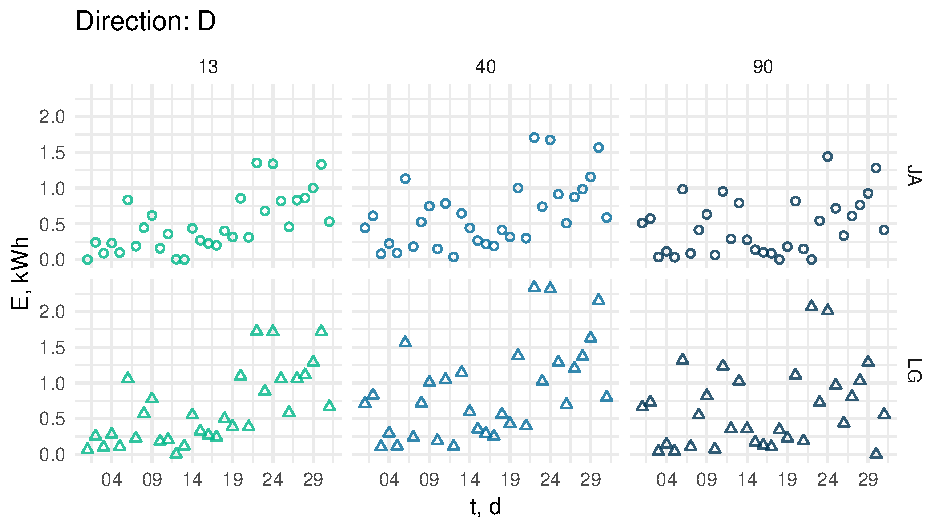
\includegraphics[width=\linewidth]{figures/mar_Deg.pdf}
    \captionof{figure}{title}
\end{center}
\begin{center}
    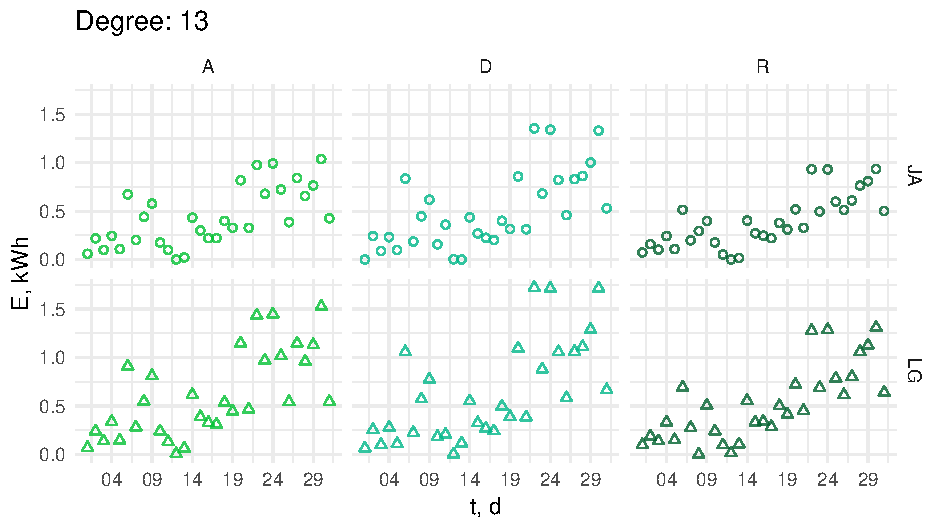
\includegraphics[width=\linewidth]{figures/mar_Dir.pdf}
    \captionof{figure}{title}
\end{center}
\begin{center}
    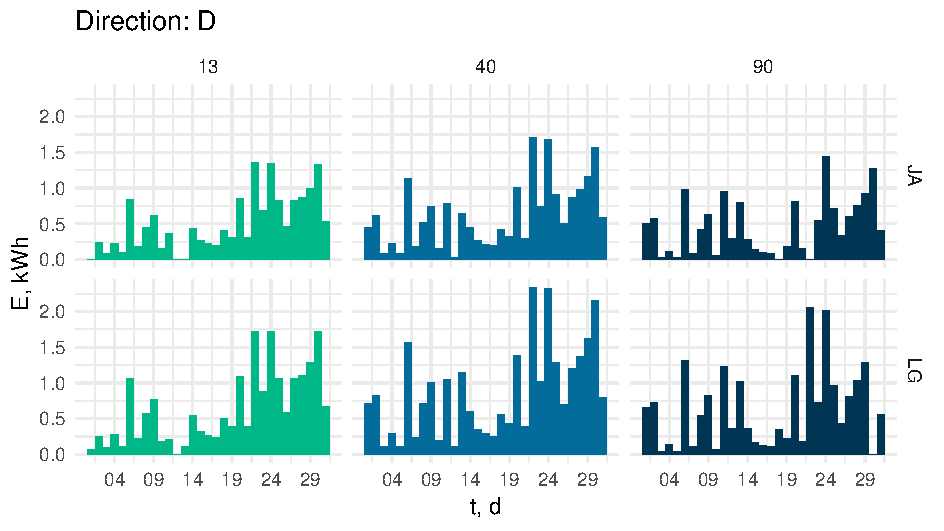
\includegraphics[width=\linewidth]{figures/mar_Degbar.pdf}
    \captionof{figure}{title}
\end{center}
\begin{center}
    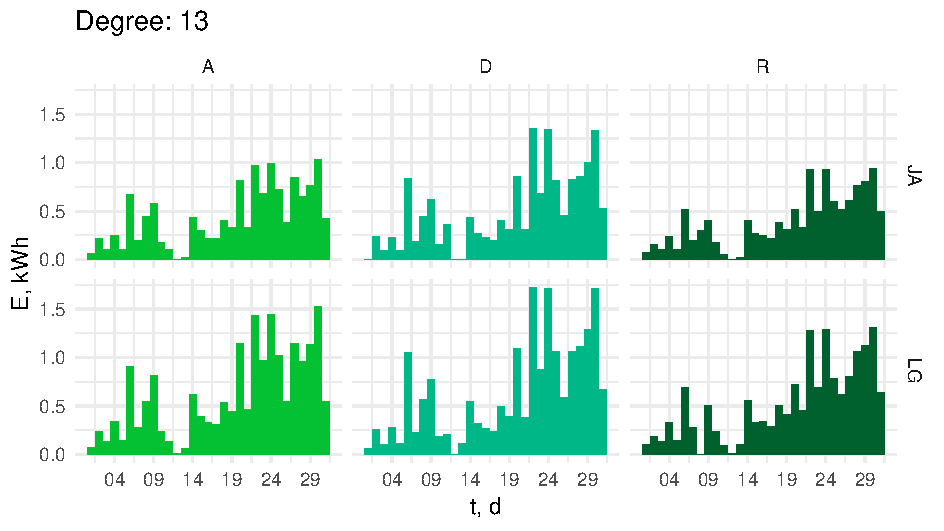
\includegraphics[width=\linewidth]{figures/mar_Dirbar.pdf}
    \captionof{figure}{title}
\end{center}
\begin{center}
    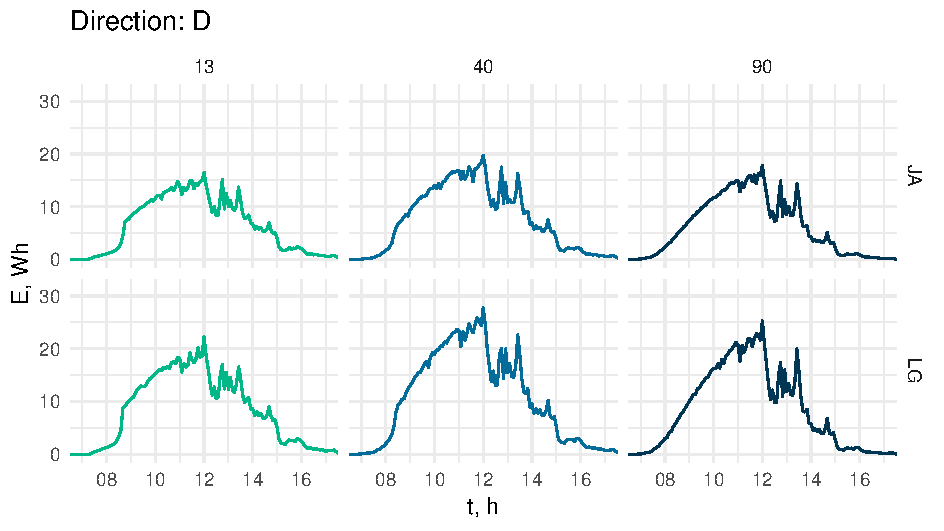
\includegraphics[width=\linewidth]{figures/mar_Deg_l.pdf}
    \captionof{figure}{title}
\end{center}
\begin{center}
    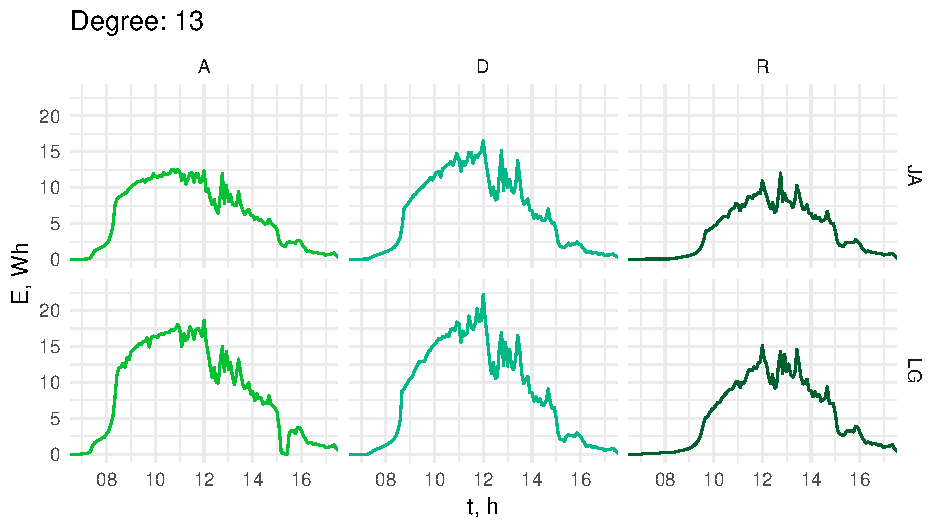
\includegraphics[width=\linewidth]{figures/mar_Dir_l.pdf}
    \captionof{figure}{title}
\end{center}
\begin{center}
    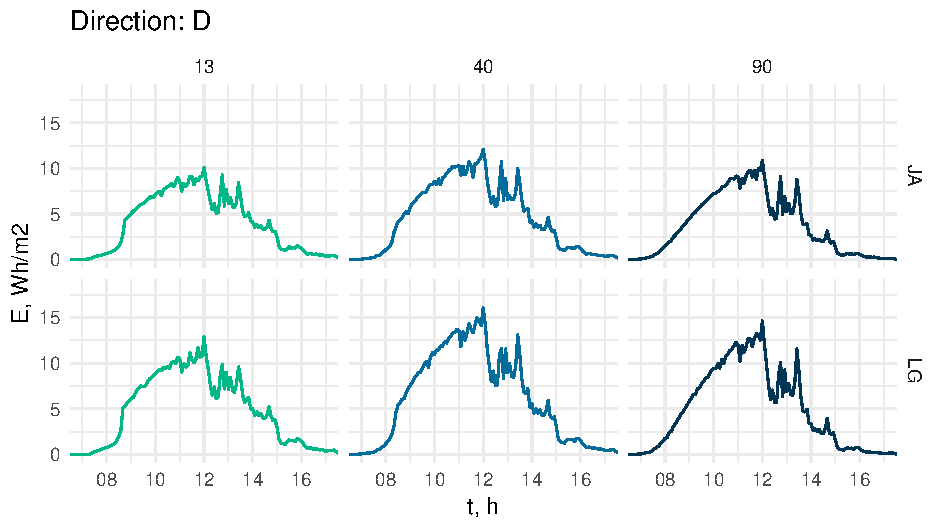
\includegraphics[width=\linewidth]{figures/mar_Deg_lm2.pdf}
    \captionof{figure}{title}
\end{center}
\begin{center}
    \includegraphics[width=\linewidth]{figures/mar_Dir_m2.pdf}
    \captionof{figure}{title}
\end{center}
\begin{center}
    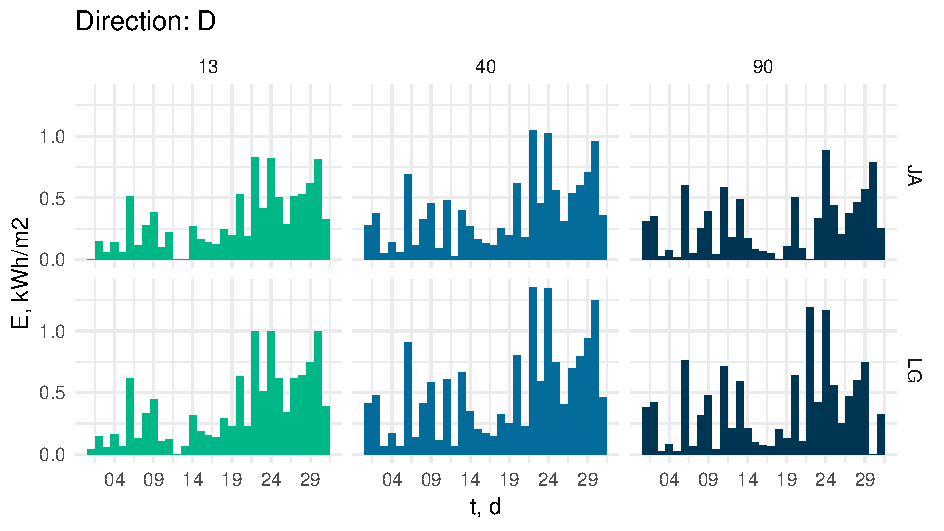
\includegraphics[width=\linewidth]{figures/mar_Degbarm2.pdf}
    \captionof{figure}{title}
\end{center}
\begin{center}
    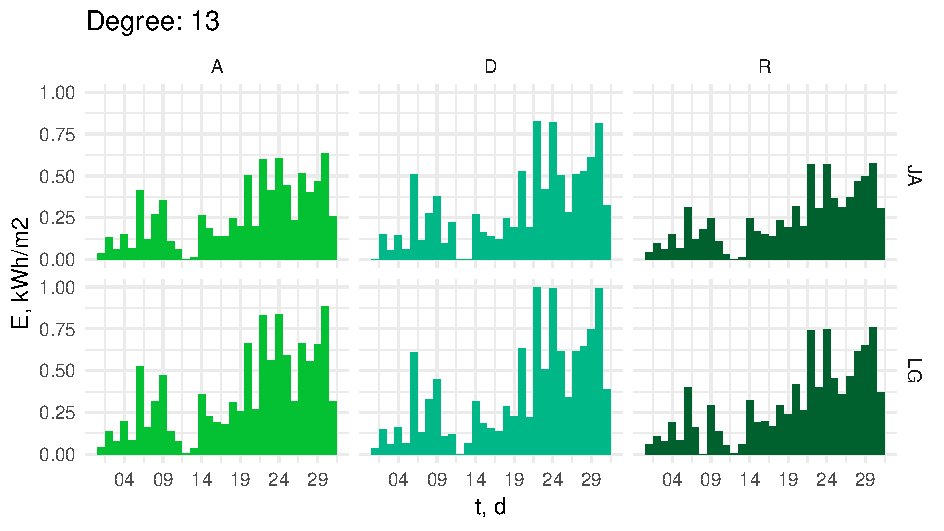
\includegraphics[width=\linewidth]{figures/mar_Dirbarm2.pdf}
    \captionof{figure}{title}
\end{center}
\begin{center}
    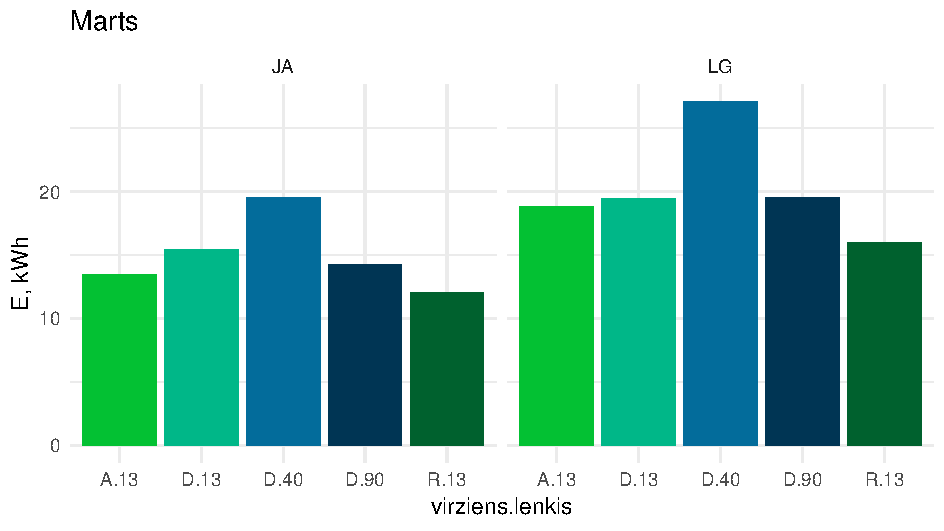
\includegraphics[width=\linewidth]{figures/mar_bar.pdf}
    \captionof{figure}{title}
\end{center}


\section{Saules paneļi}
\begin{center}
    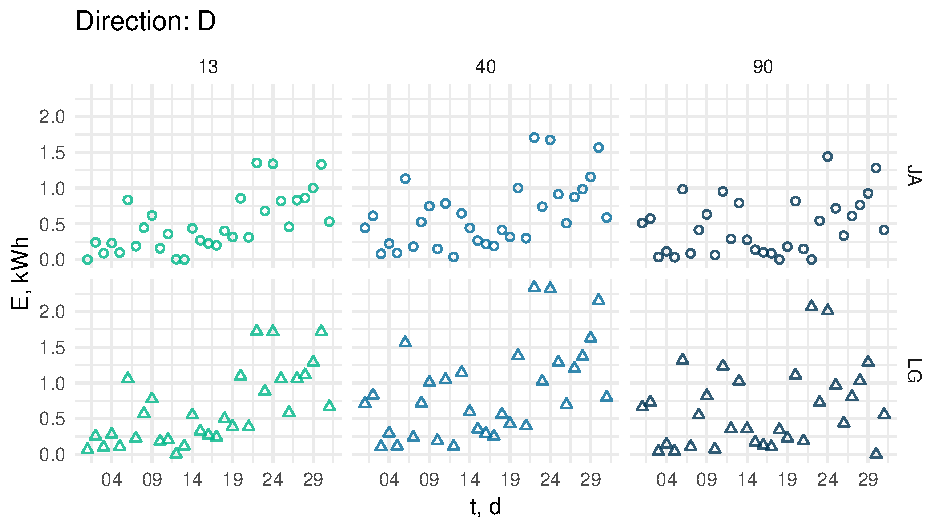
\includegraphics[width=\linewidth]{figures/mar_Deg.pdf}
    \captionof{figure}{title}
\end{center}
\begin{center}
    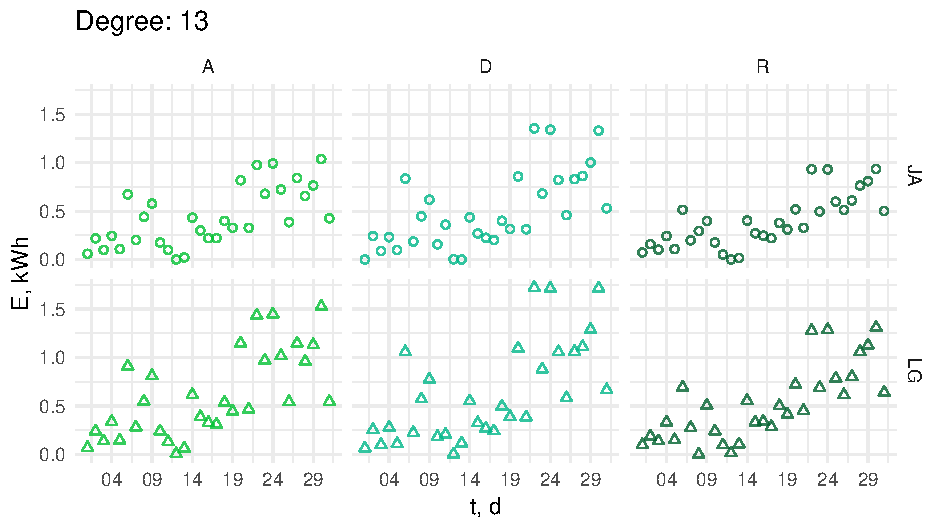
\includegraphics[width=\linewidth]{figures/mar_Dir.pdf}
    \captionof{figure}{title}
\end{center}
\begin{center}
    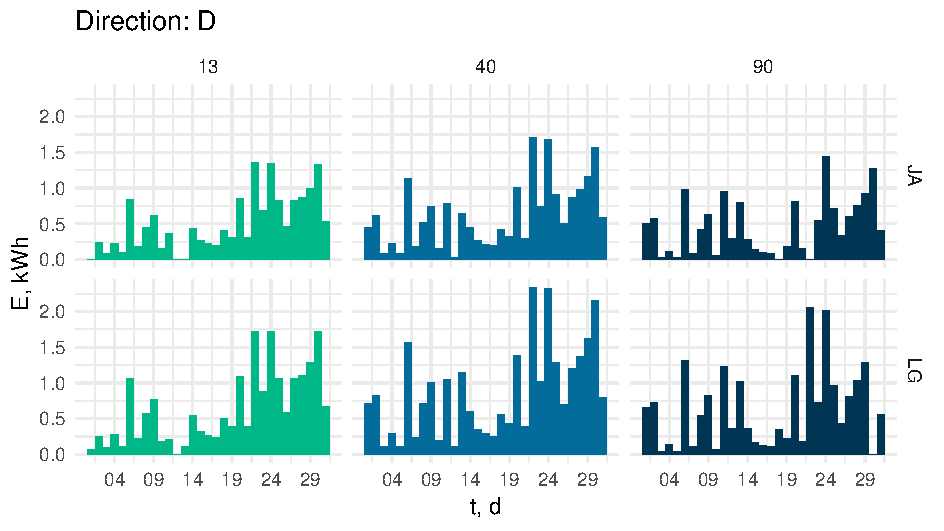
\includegraphics[width=\linewidth]{figures/mar_Degbar.pdf}
    \captionof{figure}{title}
\end{center}
\begin{center}
    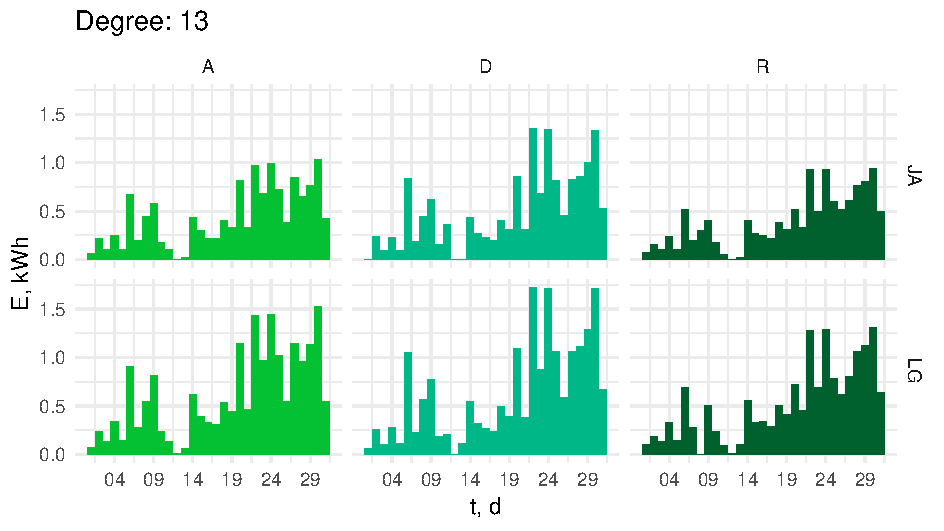
\includegraphics[width=\linewidth]{figures/mar_Dirbar.pdf}
    \captionof{figure}{title}
\end{center}
\begin{center}
    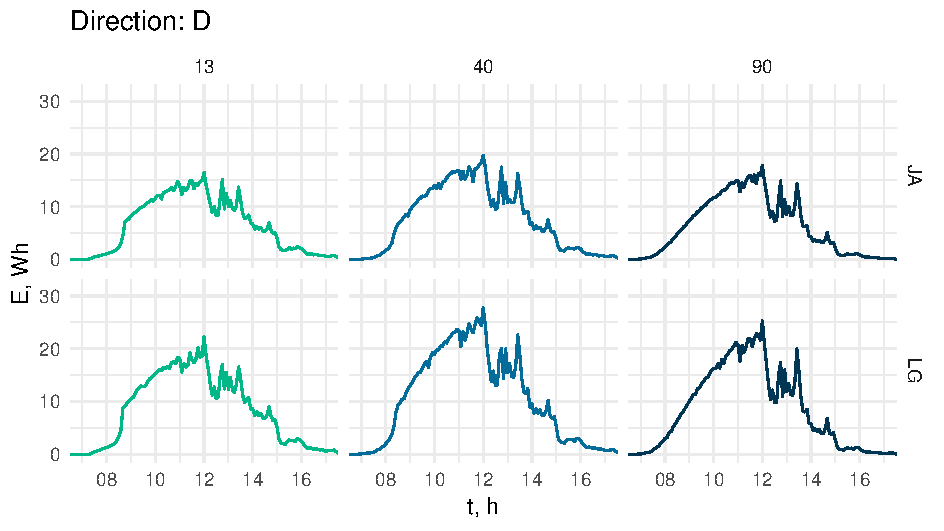
\includegraphics[width=\linewidth]{figures/mar_Deg_l.pdf}
    \captionof{figure}{title}
\end{center}
\begin{center}
    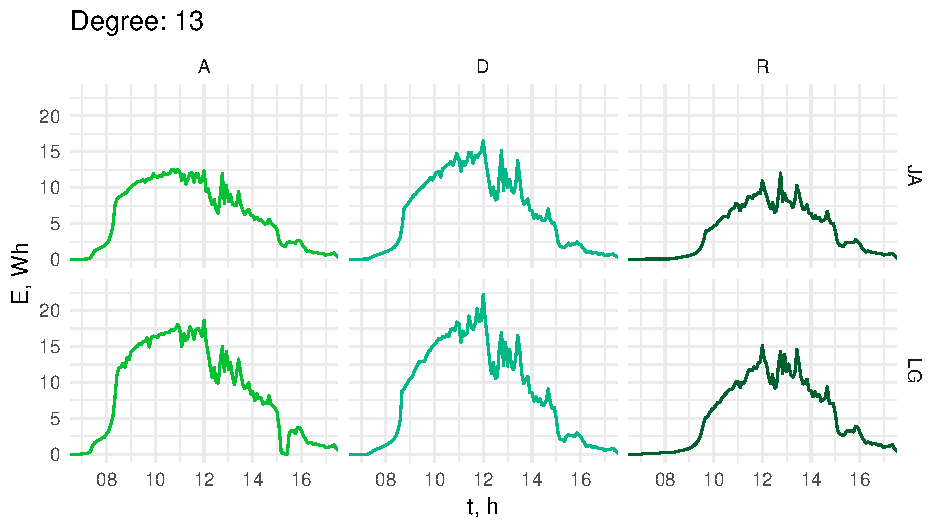
\includegraphics[width=\linewidth]{figures/mar_Dir_l.pdf}
    \captionof{figure}{title}
\end{center}
\begin{center}
    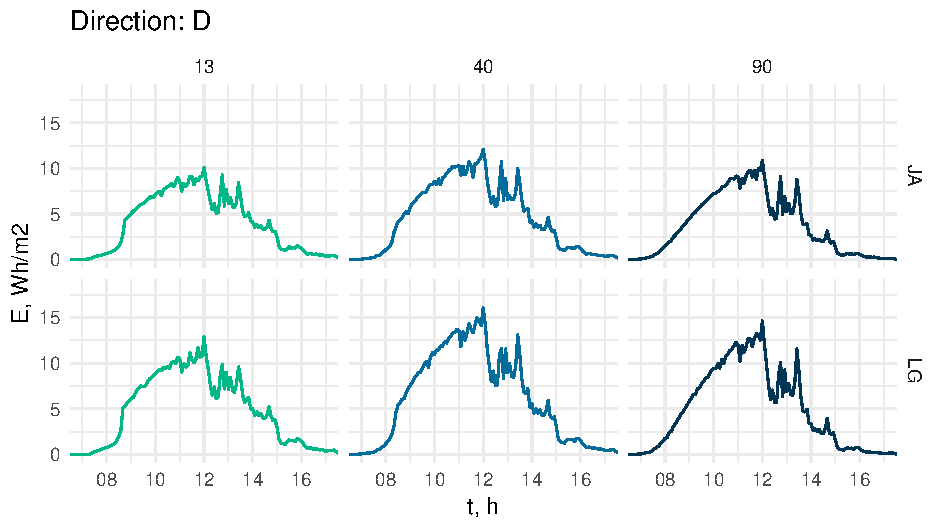
\includegraphics[width=\linewidth]{figures/mar_Deg_lm2.pdf}
    \captionof{figure}{title}
\end{center}
\begin{center}
    \includegraphics[width=\linewidth]{figures/mar_Dir_m2.pdf}
    \captionof{figure}{title}
\end{center}
\begin{center}
    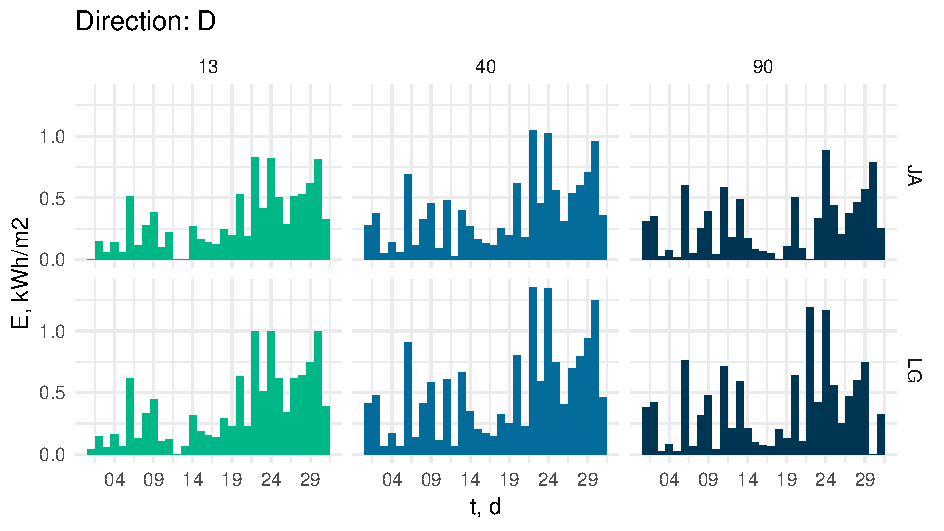
\includegraphics[width=\linewidth]{figures/mar_Degbarm2.pdf}
    \captionof{figure}{title}
\end{center}
\begin{center}
    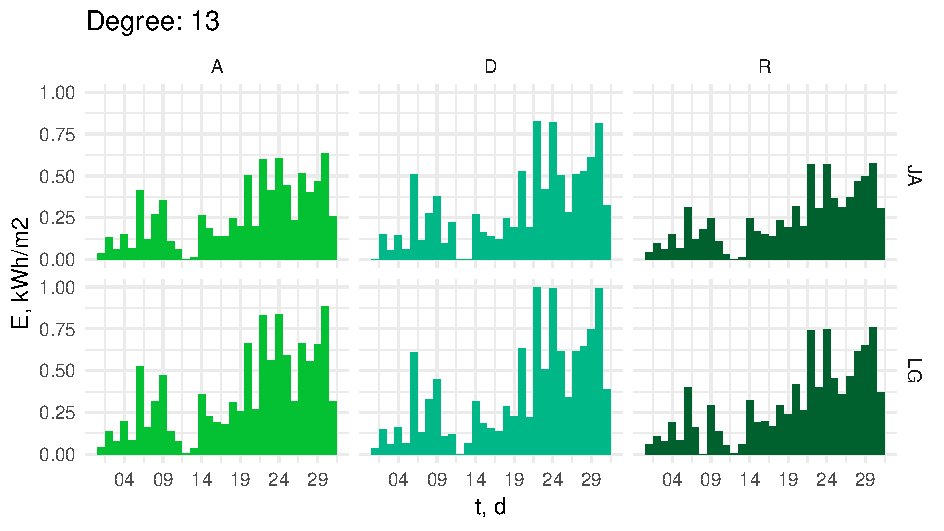
\includegraphics[width=\linewidth]{figures/mar_Dirbarm2.pdf}
    \captionof{figure}{title}
\end{center}
\begin{center}
    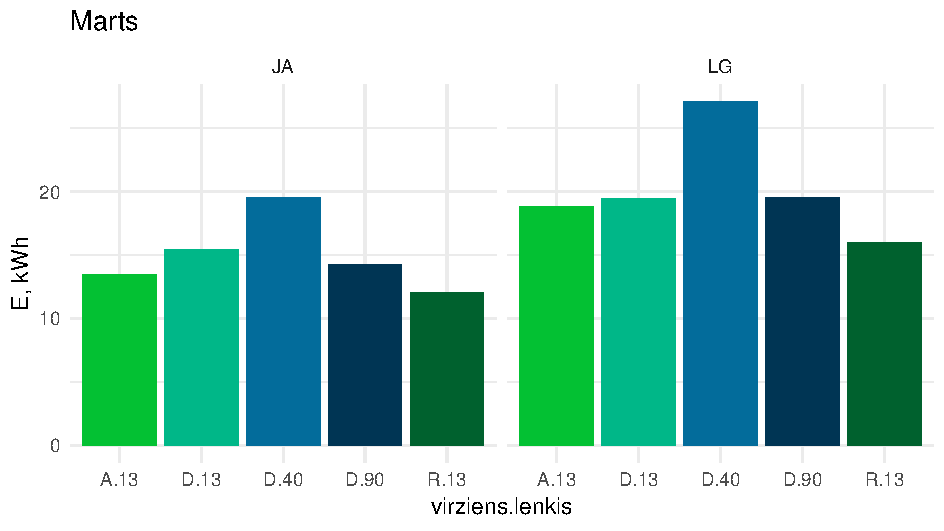
\includegraphics[width=\linewidth]{figures/mar_bar.pdf}
    \captionof{figure}{title}
\end{center}


\specnodala{Rezultāti}
Rezultāti

\specnodala{Secinājumi}
Secinājumi

% \specnodala{Pateicības}
% Pateicos paroksetīnam, xanax, GNU/Linux, Pētera Draguna dzejas krājumam 'Tumšās stundas', Tarvi Verro for teaching me git, Valtam Krūmiņam un Annai Bulei par emocionālo atbalstu, Paulīnai Lodbrukai un Pēterim Ratniekam par ticību maniem spēkiem, Žeņam par kucēnu video, Solvitai par maģiju un Cilvēkam par pacietību. Paldies Aleksandrai Elbakjanai par sci-hub. Paldies "Puratos Latvia" un Asjas un Berndta Everts piemiņas fondam par stipendiju studiju laikā.\\

Darbs veikts ar Eiropas Reģionālās attīstības fonta projekta "Viedo risinājumu gandrīz nulles enerģijas ēkām izstrāde, optimizācija un ilgtspējas izpēte reāla klimata apstākļos" Nr ESS2017/209 1.1.1.1/16/A/192 finansiālo atbalstu.


% \literatura{main.bib}
% \bibliography{main.bib}

\bibliographystyle{bakd}
\phantomsection
\renewcommand{\bibname}{Izmantotā literatūra un avoti}
\renewcommand{\refname}{\bibname}
% \addcontentsline{toc}{chapter}{\bibname}
\bibliography{main.bib}

% \appendix
% \chapter{Izveidoto programmu kods}
% \input{pielikumi/kods1.tex}

\end{document}
